\documentclass{exam}

\usepackage{units} 
\usepackage{graphicx}
\usepackage[fleqn]{amsmath}
\usepackage{cancel}
\usepackage{float}
\usepackage{mdwlist}
\usepackage{booktabs}
\usepackage{cancel}
\usepackage{polynom}
\usepackage{caption}
\usepackage{fullpage}
\usepackage{comment}
\usepackage{enumerate}
\usepackage{xfrac}

\newcommand{\degree}{\ensuremath{^\circ}} 
\everymath{\displaystyle}

% \begin{figure}[H]
%   \centering
%   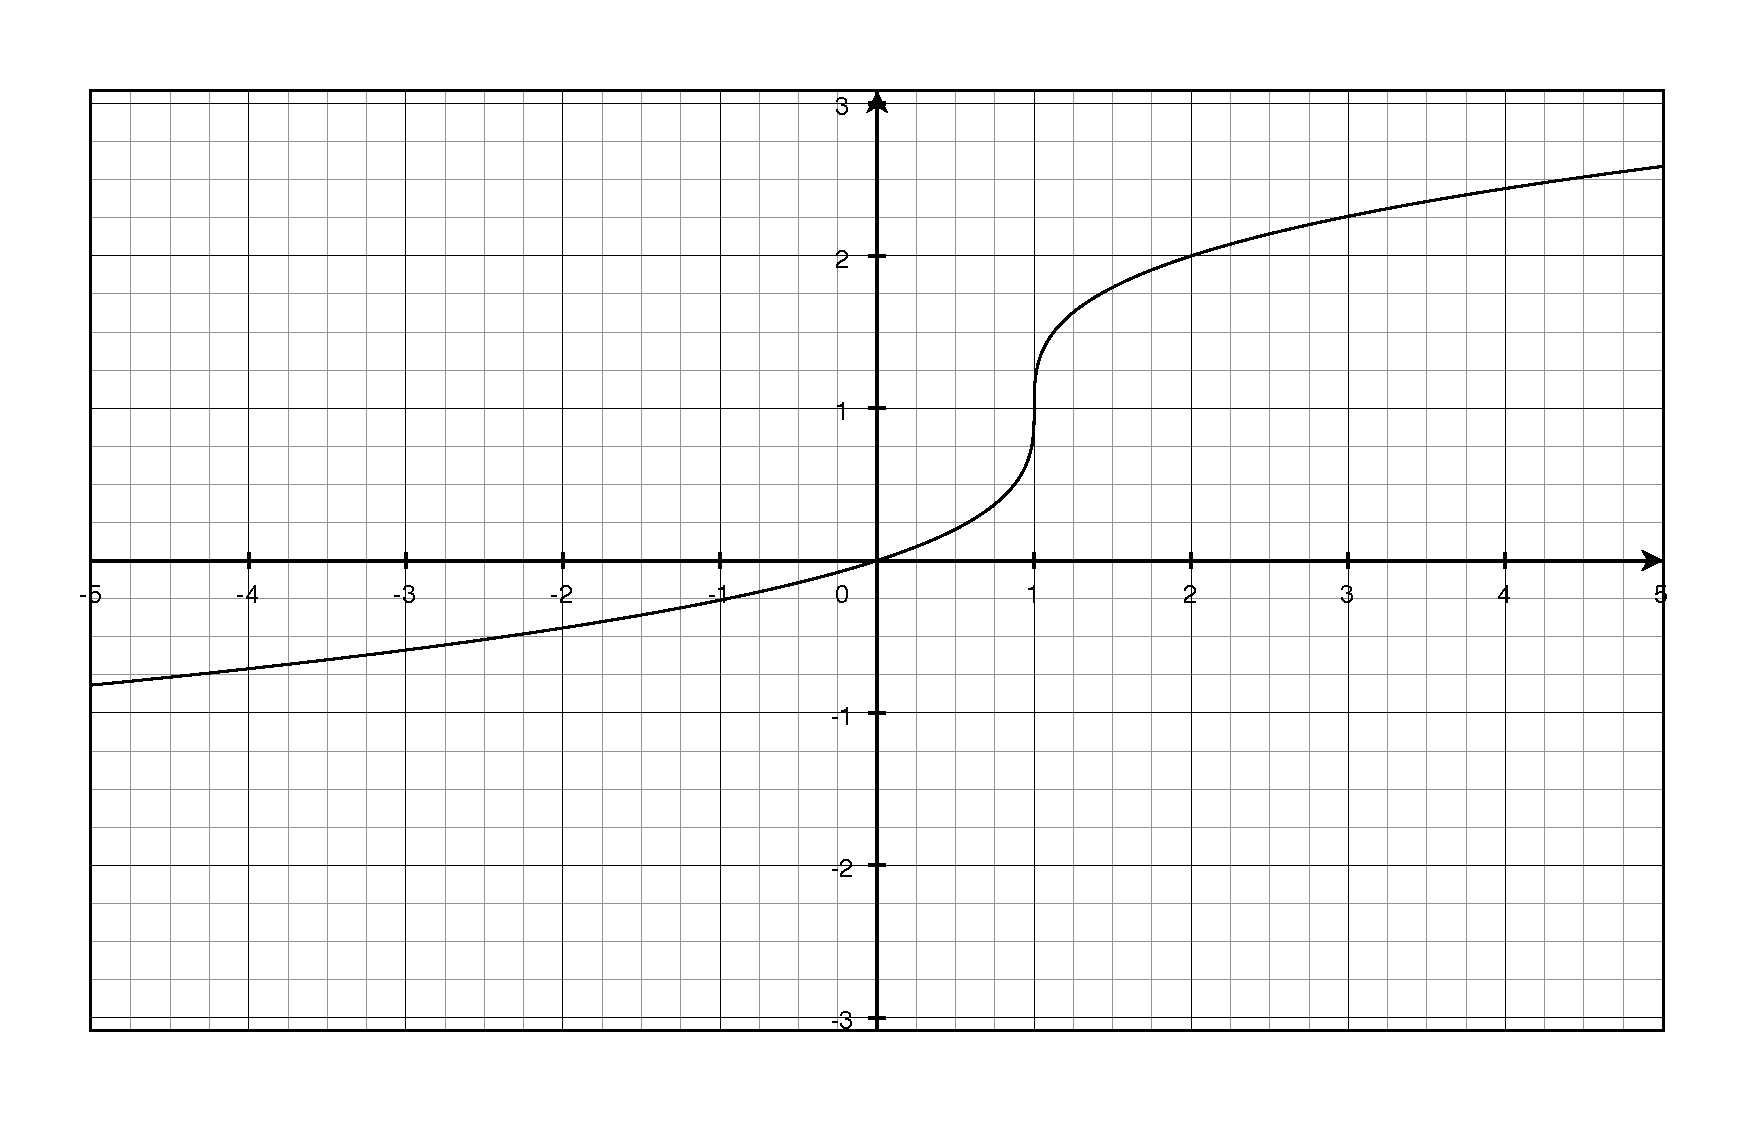
\includegraphics[scale=.3]{question7.eps}
%   \caption*{question 7}
% \end{figure}

% \begin{tabular}{cc}
%   \toprule
%   period & amplitude \\
%     $\pi$ & $2$ \\
%   \bottomrule
% \end{tabular}

\printanswers
\excludecomment{comment}

\ifprintanswers 
  \usepackage{2in1, lscape} 
\fi

\author{}
\date{\today}
\title{Math 142 \\ Homework Seven}

\begin{document}

  \maketitle

  \section{Homework}
  Section 6.2: 

  \section{Extra Credit}
  Section 6.2: TO DO

  \ifprintanswers

    \section{Section 6.1}
    \begin{description}

      \item[1] 
        \begin{tabular}[H]{cccccc}
          \toprule
          $\sin$         & $\cos$         & $\tan$         & $\sec$         & $\csc$         & $\cot$ \\
          % \midrule
          $\sfrac{4}{5}$ & $\sfrac{3}{5}$ & $\sfrac{4}{3}$ & $\sfrac{5}{3}$ & $\sfrac{5}{4}$ & $\sfrac{3}{4}$ \\
          \bottomrule
        \end{tabular}

      \item[2] 
        \begin{tabular}[H]{cccccc}
          \toprule
          $\sin$          & $\cos$           & $\tan$          & $\sec$           & $\csc$          & $\cot$ \\
          % \midrule
          $\sfrac{7}{25}$ & $\sfrac{24}{25}$ & $\sfrac{7}{24}$ & $\sfrac{25}{24}$ & $\sfrac{25}{7}$ & $\sfrac{24}{7}$ \\
          \bottomrule
        \end{tabular}

      \item[3] 
        Find the missing side:
        \begin{align*}
          x^2 + 40^2 & = 41^2 \\
          x          & = 9 \\
        \end{align*}

        \begin{tabular}[H]{cccccc}
          \toprule
          $\sin$          & $\cos$           & $\tan$          & $\sec$           & $\csc$          & $\cot$ \\
          % \midrule
          $\sfrac{40}{41}$ & $\sfrac{9}{41}$ & $\sfrac{40}{9}$ & $\sfrac{41}{9}$ & $\sfrac{41}{40}$ & $\sfrac{9}{40}$ \\
          \bottomrule
        \end{tabular}

      \item[4] 
        Find the missing side:
        \begin{align*}
          15^2 + 8^2 & = r^2 \\
          r          & = 17 \\
        \end{align*}

        \begin{tabular}[H]{cccccc}
          \toprule
          $\sin$          & $\cos$           & $\tan$          & $\sec$           & $\csc$          & $\cot$ \\
          % \midrule
          $\sfrac{15}{17}$ & $\sfrac{8}{17}$ & $\sfrac{15}{8}$ & $\sfrac{17}{8}$ & $\sfrac{17}{15}$ & $\sfrac{8}{15}$ \\
          \bottomrule
        \end{tabular}

      \item[5] 
        Find the missing side:
        \begin{align*}
          3^2 + 2^2 & = r^2 \\
          r         & = \sqrt{13} \\
        \end{align*}

        \begin{tabular}[H]{cccccc}
          \toprule
          $\sin$          & $\cos$           & $\tan$          & $\sec$           & $\csc$          & $\cot$ \\
          % \midrule
          $\sfrac{2}{\sqrt{13}}$ & $\sfrac{3}{\sqrt{13}}$ & $\sfrac{2}{3}$ & $\sfrac{\sqrt{13}}{3}$ & $\sfrac{\sqrt{13}}{2}$ & $\sfrac{3}{2}$ \\
          \bottomrule
        \end{tabular}

      \item[6] 
        Find the missing side:
        \begin{align*}
          x^2 + 7^2 & = 8^2 \\
          x         & = \sqrt{15} \\
        \end{align*}

        \begin{tabular}[H]{cccccc}
          \toprule
          $\sin$          & $\cos$           & $\tan$          & $\sec$           & $\csc$          & $\cot$ \\
          % \midrule
          $\sfrac{7}{8}$ & $\sfrac{\sqrt{15}}{8}$ & $\sfrac{7}{\sqrt{15}}$ & $\sfrac{8}{\sqrt{15}}$ & $\sfrac{8}{7}$ & $\sfrac{\sqrt{15}}{7}$ \\
          \bottomrule
        \end{tabular}

      \item[7]
        Find the missing side:
        \begin{align*}
          3^2 + 5^2 & = r^2 \\
          x         & = \sqrt{34} \\
        \end{align*}

        \begin{align*}
          \sin \alpha & = \cos \beta = \frac{3}{\sqrt{34}} \\
          \tan \alpha & = \cot \beta = \frac{3}{5} \\
          \sec \alpha & = \csc \beta = \frac{\sqrt{34}}{5} \\
        \end{align*}

      \item[8]
        Find the missing side:
        \begin{align*}
          x^2 + 4^2 & = 7^2 \\
          x         & = \sqrt{33} \\
        \end{align*}

        \begin{align*}
          \sin \alpha & = \cos \beta = \frac{4}{7} \\
          \tan \alpha & = \cot \beta = \frac{4}{\sqrt{33}} \\
          \sec \alpha & = \csc \beta = \frac{7}{4} \\
        \end{align*}

      \item[9]
        \begin{align*}
          \sin 30 \degree & = \frac{x}{25} \\
          \frac{1}{2}     & = \frac{x}{25} \\
          x               & = \frac{25}{2} \\
        \end{align*}

      \item[10]
        \begin{align*}
          \sin 45 \degree    & = \frac{12}{x} \\
          \frac{\sqrt{2}}{2} & = \frac{12}{x} \\
          x                  & = \boxed{ 12 \sqrt{2} } \\
        \end{align*}

      \item[11]
        \begin{align*}
          \sin 60 \degree    & = \frac{x}{13} \\
          \frac{\sqrt{3}}{2} & = \frac{x}{13} \\
          x                  & = \boxed{ \frac{13 \sqrt{3}}{2} } \\
        \end{align*}

      \item[12]
        \begin{align*}
          \tan 30 \degree    & = \frac{4}{x} \\
          \frac{\sqrt{3}}{3} & = \frac{4}{x}  \\
          x                  & = \boxed{ 4 \sqrt{3} } \\
        \end{align*}

      \item[15]
        \begin{align*}
          \sin \theta & = \frac{y}{28} \\
          y           & = \boxed{ 28 \sin \theta } \\
          \\
          \cos \theta & = \frac{x}{28} \\
          x           & = \boxed{ 28 \cos \theta } \\
        \end{align*}

      \item[16]
        \begin{align*}
          \tan \theta & = \frac{x}{4} \\
          x           & = \boxed{ 4 \tan \theta } \\
          \\
          \sec \theta & = \frac{y}{4} \\
          y           & = \boxed{ 4 \sec \theta } \\
        \end{align*}

      \item[17] 
        Find the missing side:
        \begin{align*}
          x^2 + 3^2 & = 5^2 \\
          x         & = 4 \\
        \end{align*}

        \begin{tabular}[H]{cccccc}
          \toprule
          $\sin$          & $\cos$           & $\tan$          & $\sec$           & $\csc$          & $\cot$ \\
          $\sfrac{4}{5}$ & $\sfrac{3}{5}$ & $\sfrac{4}{3}$ & $\sfrac{5}{3}$ & $\sfrac{5}{4}$ & $\sfrac{3}{4}$ \\
          \bottomrule
        \end{tabular}

      \item[18] 
        Find the missing side:
        \begin{align*}
          9^2 + y^2 & = 40^2 \\
          x         & = 7 \sqrt{31} \\
        \end{align*}

        \begin{tabular}[H]{cccccc}
          \toprule
          $\sin$                    & $\cos$          & $\tan$                   & $\sec$          & $\csc$                    & $\cot$ \\
          $\sfrac{7 \sqrt{91}}{40}$ & $\sfrac{9}{40}$ & $\sfrac{7 \sqrt{91}}{9}$ & $\sfrac{40}{9}$ & $\sfrac{40}{7 \sqrt{91}}$ & $\sfrac{9}{7 \sqrt{91}}$ \\
          \bottomrule
        \end{tabular}

      \item[23]
        \begin{align*}
          \sin \frac{\pi}{6} + \cos \frac{\pi}{6} & = \frac{1}{2} + \frac{\sqrt{3}}{2} \\
                                                  & = \boxed{ \frac{1 + \sqrt{3}}{2} } \\
        \end{align*}

      \item[24]
        \begin{align*}
          \sin 30 \degree + \csc 30 \degree & = \frac{1}{2} + 2 \\
                                            & = \boxed{ \frac{5}{2} } \\
        \end{align*}

      \item[25]
        \begin{align*}
          \sin 30 \degree \cos 60 \degree + \sin 60 \degree \cos 30 \degree               & =
            \frac{1}{2} \times \frac{1}{2} + \frac{\sqrt{3}}{2} \times \frac{\sqrt{3}}{2} \\
                                                                                          & = \frac{1}{4} + \frac{3}{4} \\
                                                                                          &= \boxed{ 1 } \\
        \end{align*}

      \item[26]
        \begin{align*}
          ( \sin 60 \degree )^2 + ( \cos 60 \degree )^2 & = ( \frac{\sqrt{3}}{2} )^2 + ( \frac{1}{2} )^2 \\
                                                        & = \frac{3}{4} + \frac{1}{4} \\
                                                        & = \boxed{ 1 } \\
        \end{align*}

    \end{description}

  \else
    \vspace{1 cm}
    \begin{quote}
      \begin{em}
        TO DO
      \end{em}
    \end{quote}
    \hspace{1 cm} --Shunryu Suzuki
  \fi

\end{document}

